\subsection{METRIZABLE SPACES OF COUNTABLE TYPE}

DEFINITION 4. A metrizable space is said to be of countable type (or separable) if its topology has a countable base.

Clearly every subspace of a metrizable space of countable type is again of countable type. The definition of the base of the topology of a product space (Chapter I, § 4, no. 1) and Corollary 2 to Theorem 1 of no. 4 show that the product of a countable family of metrizable spaces of countable type is a metrizable space of countable type. Again, the sum of a countable family of metrizable spaces of countable type is a metrizable space of countable type (no. 5).

PROPOSITION 12. If X is a metrizable topological space, the following statements are equivalent:

\begin{enumerate}
\def\labelenumi{\alph{enumi})}
\item
  X is of countable type.
\item
  X has a countable dense subset.
\item
  X is homeomorphic to a subspace of the cube IN, where I is the interval {[}o, i{]} in R.
\end{enumerate}

From the preceding remarks it is clear that c) implies a); a) implies b), for if \((\mathbf{U}_{n})\) is a countable base of the topology of X and \(a_{n}\) is a point of \(U_{n}\) , the \(a_{n}\) form a dense subset of X. Finally let us show that b) implies c). Let \((a_{n})\) be a dense sequence of points of X, and for each \(x \in X\) let \(\varphi(x)\) be the point \((d(x, a_{n}))_{n \in \mathbb{N}}\) of \(I^{N}\) (d being a metric compatible with the topology of X, with respect to which the diameter of X is \(\leqslant 1\) ). We shall show that \(\varphi\) is a homeomorphism of X onto a subspace of \(I^{N}\) . Indeed, \(\varphi\) is continuous, because each of the functions \(x \to d(x, a_{n})\) is continuous; and \(\varphi\) is injective, because each point of X is the limit of some subsequence of \((a_{n})\) (Proposition 8). Let B be a ball with centre \(x_{0}\) and radius r in X, and let n be an integer such that

\[
\left| d (x _ {0}, a _ {n}) <   \frac {1}{3} r. \right|
\]

The image under \(\varphi\) of the set \(W\) of points \(x\in X\) such that

\[
\left| d (x _ {0}, a _ {n}) - d (x, a _ {n}) \right| <   \frac {1}{3} r
\]

is by definition a neighbourhood of \(\varphi(x_0)\) in \(\varphi(\mathbf{X})\) . But for each \(x \in W\) we have \(d(x, a_n) < d(x_0, a_n) + \frac{1}{3} r < \frac{2}{3} r\) , whence

\[
d (x, x _ {0}) \leqslant d (x _ {0}, a _ {n}) + d (x, a _ {n}) <   r,
\]

which shows that W is a neighbourhood of \(x_{0}\) contained in B, and therefore that \(\varphi\) is a homeomorphism of X onto \(\varphi(\mathbf{X})\) .

\pandocbounded{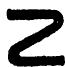
\includegraphics[keepaspectratio]{images/part001_a8399183.jpg}}

Note that for an arbitrary topological space X, property b) does not necessarily imply the existence of a countable base, even if X is compact and every point of X has a countable fundamental system of neighbourhoods (Exercise 13; cf.~Chapter I, § 1, Exercise 7).

PROPOSITION 13. Let X be a topological space which has a countable base \((\mathbf{U}_n)\) ; then for each open covering \((\mathbf{V}_t)_{i \in \mathbf{I}}\) of X there exists a countable subset J of I such that \((\mathbf{V}_t)_{i \in \mathbf{J}}\) is a covering of X.

Let H be the subset of N consisting of indices n such that \(U_{n}\) is contained in at least one of the \(V_{t}\) ; the sequence \((\mathrm{U}_{n})_{n\in\mathbf{H}}\) is a covering of X, because every point \(x\in X\) belongs to some \(V_{t}\) , and since \(V_{t}\) is open, there is an index n such that \(x\in U_{n}\subset V_{t}\) . Hence there is a mapping \(\psi\) of H into I such that \(U_{n}\subset V_{\psi(n)}\) for each \(n\in H\) ; taking \(J=\psi(H)\) , which is countable, the proposition is proved.

